% This is samplepaper.tex, a sample chapter demonstrating the
% LLNCS macro package for Springer Computer Science proceedings;
% Version 2.20 of 2017/10/04
%
\documentclass[runningheads]{llncs}
%
\usepackage{graphicx}
% Used for displaying a sample figure. If possible, figure files should
% be included in EPS format.
%
% If you use the hyperref package, please uncomment the following line
% to display URLs in blue roman font according to Springer's eBook style:
% \renewcommand\UrlFont{\color{blue}\rmfamily}

\begin{document}
%
\title{Stroke Prediction Capstone Project}
%
%\titlerunning{Abbreviated paper title}
% If the paper title is too long for the running head, you can set
% an abbreviated paper title here
%
\author{Alvaro Quintero Gonzalez}
%
\authorrunning{A. Quintero Gonzalez.}
% First names are abbreviated in the running head.
% If there are more than two authors, 'et al.' is used.
%
\institute{Northwest Missouri State University, Maryville MO 64468, USA \\
\email{S573928@nwmissouri.edu and alvaroquintero28@yahoo.com}}
%
\maketitle              % typeset the header of the contribution
%
\begin{abstract}
Stroke prediction is a critical area of research in healthcare, aiming to enhance preventative strategies and improve patient outcomes. This study investigates a comprehensive dataset collected from various healthcare sources, consisting of demographic, clinical, and lifestyle factors associated with stroke risk. The dataset encompasses attributes such as age, gender, blood pressure, cholesterol levels, body mass index (BMI), and lifestyle habits. Utilizing machine learning algorithms, we apply classification techniques—including logistic regression, decision trees, and random forests—to identify significant predictors of stroke occurrence. Analysis reveals that key factors such as hypertension, diabetes, and smoking significantly increase stroke risk, while regular physical activity acts as a protective measure. The insights gained from this study can guide healthcare professionals in stratifying patients based on their risk profiles and recommending tailored preventative measures. Additionally, findings emphasized the importance of addressing modifiable risk factors in public health initiatives. This research not only contributes to the existing body of literature on stroke prediction but also underscores the potential for machine learning to revolutionize patient care and stroke prevention strategies in clinical practice.

\keywords{Stroke Prediction \and Preventative Strategies \and Demographic Factors \and Predictive Modeling \and Machine Learning Algorithms}
\end{abstract}
%
%
%
\section{Introduction}

Strokes are a major health concern globally, recognized as one of the leading causes of disability and death. Occurring when blood flow to the brain is disrupted, it can lead to significant physical, cognitive, and emotional impairments in affected individuals. \cite{kaur2022retracted} The impact of strokes extends beyond the individual, affecting families and communities, and placing a substantial strain on healthcare systems. With the rising incidence of strokes associated with aging populations and the increasing prevalence of risk factors such as hypertension, obesity, and diabetes, there is an urgent need to focus on effective stroke prevention strategies. Prevention requires a multifaceted approach that includes public education, early identification of risk factors, and lifestyle modifications. Simple changes, such as adopting a balanced diet, engaging in regular physical activity, and managing underlying health conditions, can greatly reduce an individual's risk of stroke. Moreover, healthcare providers must play an active role in raising awareness about stroke prevention and ensuring that at-risk patients receive appropriate screenings and interventions. By promoting a comprehensive understanding of stroke risk factors, we can empower individuals to take charge of their health. This proactive approach not only aims to reduce the frequency of strokes but also facilitates overall public health awareness, fostering healthier communities. As advances in knowledge and strategies for stroke prevention, we can work towards a future where strokes are less frequent and their consequences are minimized \cite{sirisha2021awareness}.

Subsequent paragraphs, however, are indented.

\subsection{Goals of this Capstone Project} 
Specify exactly your aims of this paper. Also, write a sentence how you will address for each individual goal.

\subsection{This is another subsection}
Write something related to your paper.

\section{Data}


\begin{table}
\caption{Gas Prices}\label{gasprice}
\begin{tabular}{|l|r|}
\hline
Month &  Price \\
\hline
Jan &  \$2.12 \\
Feb &  0.12 \% \\
\hline
Mar &  1.12 \\
\hline
Apr &  2.12 \\
May &  3.12 \\
Jun &  1.12 \\

\hline
\end{tabular}
\end{table}



\begin{table}
\caption{Table captions should be placed above the
tables.}\label{tab1}
\begin{tabular}{|l|l|l|}
\hline
Heading level &  Example & Font size and style\\
\hline
Title (centered) &  {\Large\bfseries Lecture Notes} & 14 point, bold\\
1st-level heading &  {\large\bfseries 1 Introduction} & 12 point, bold\\
2nd-level heading & {\bfseries 2.1 Printing Area} & 10 point, bold\\
3rd-level heading & {\bfseries Run-in Heading in Bold.} Text follows & 10 point, bold\\
4th-level heading & {\itshape Lowest Level Heading.} Text follows & 10 point, italic\\
\hline
\end{tabular}
\end{table}


The gasoline prices are summarized in Table \ref{gasprice}



\noindent Displayed equations are centered and set on a separate
line.
\begin{equation}
x + y = z
\end{equation}
Please try to avoid rasterized images for line-art diagrams and
schemas. Whenever possible, use vector graphics instead (see
Fig.~\ref{fig1}).

\begin{figure}
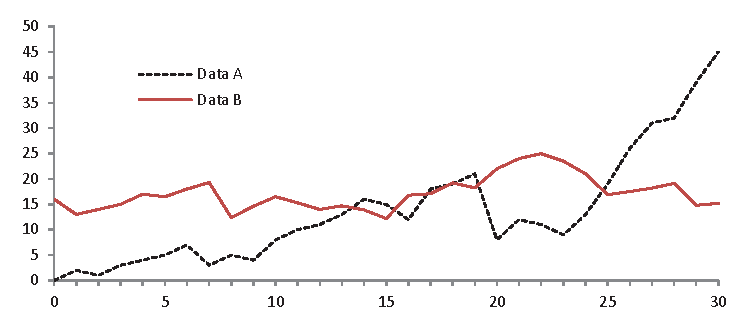
\includegraphics[width=\textwidth]{fig1.eps}
\caption{A figure caption is always placed below the illustration.
Please note that short captions are centered, while long ones are
justified by the macro package automatically.} 
\label{fig1}
\end{figure}

The detailed steps of the MEC is shown in Figure \ref{mecFig}.

\begin{figure}
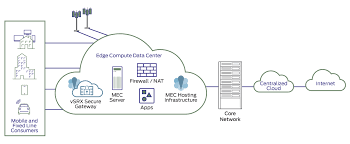
\includegraphics[width=\textwidth]{mecomputing.png}
\caption{This is the MEC} 
\label{mecFig}
\end{figure}

%\begin{theorem}
%This is a sample theorem. The run-in heading is set in bold, while
%the following text appears in italics. Definitions, lemmas,
%propositions, and corollaries are styled the same way.
%\end{theorem}
%
% the environments 'definition', 'lemma', 'proposition', 'corollary',
% 'remark', and 'example' are defined in the LLNCS documentclass as well.
%
\begin{proof}
Proofs, examples, and remarks have the initial word in italics,
while the following text appears in normal font.
\end{proof}


The following are the items in my lunch menu.
\begin{itemize}
    \item Fish
    \begin{itemize}
        \item sauce
        \item fires
    \end{itemize}
    \item Chicken
    \item Yogurt
    \item ice cream
\end{itemize}


The following are the phases of project implementation. 
\begin{enumerate}
\item Define the Problem and Objectives
\begin{enumerate}
    \item Clearly articulate the specific questions and objectives of the analysis, focusing on how heart disease predictions can improve preventive measures for stroke patients.
    \item Identify key performance indicators (KPIs) to measure the success of the project. 
\end{enumerate}
\item  Literature Review and Background Research
\begin{enumerate}
    \item Conduct a thorough review of existing literature on heart disease, stroke rehabilitation, and predictive analytics in healthcare. 
    \item Gather insights into current best practices and identify gaps in the existing research that your project can address. 
\end{enumerate}
\item Data Collection
\begin{enumerate}
    \item Search for relevant datasets using the identified sources (e.g., ProjectPro, American Journal of Medicine) focusing on: 
    \begin{enumerate}
        \item Patient demographics 
        \item Medical history related to heart disease and strokes 
        \item Lifestyle factors (e.g., diet, exercise) 
        \item Laboratory test results (e.g., cholesterol levels, blood pressure) 
    \end{enumerate}
    \item Ensure that the data is reliable, accurate, and representative of the population you wish to study. 
\end{enumerate}
\item Data Preprocessing
    \begin{enumerate}
        \item Clean the data by handling missing values, outliers, and inconsistencies. 
        \item Perform data normalization or standardization if necessary. 
        \item Encode categorical variables to facilitate analysis in machine learning models. 
    \end {enumerate}
\item  Exploratory Data Analysis (EDA)
    \begin{enumerate}
        \item Analyze the dataset to uncover patterns and relationships between variables. 
        \item Use visualizations (graphs, plots) to represent findings and identify key risk factors associated with heart disease in stroke patients. 
    \end{enumerate}
\item Feature Selection
\begin{enumerate}
    \item Identify and select the most relevant features that influence heart disease predictions. 
    \item Use techniques like correlation analysis, recursive feature elimination (RFE), or machine learning algorithms to enhance feature selection. 
\end{enumerate}
\item Model Development
    \begin{enumerate}
        \item Choose appropriate machine learning models for prediction, such as: 
            \begin{enumerate}
                \item \item Logistic Regression
                \item Decision Trees 
                \item Random Forest 
                \item Support Vector Machines 
                \item Neural Networks 
            \end{enumerate}
        \item Split the dataset into training and testing sets for model evaluation. 
    \end{enumerate}
\item Model Training and Tuning
    \begin{enumerate}
        \item Train the selected models on the training dataset. 
        \item Optimize model performance using techniques like hyperparameter tuning and cross-validation to prevent overfitting. 
    \end{enumerate}
\item Model Evaluation
\begin{enumerate}
    \item Assess the accuracy and effectiveness of the models using the testing dataset. 
    \item Use evaluation metrics such as accuracy, precision, recall, F1 score, and the ROC-AUC curve to measure performance. 
    \item Compare the performance of different models to select the best one. 
\end{enumerate}
\item Conclusion
\begin{enumerate}
    \item Interpret Results
        \begin{enumerate}
            \item Analyze the results of the best-performing model to understand the impact of various factors on heart disease predictions. 
            \item Provide actionable insights and recommendations for preventing heart disease in stroke patients based on the findings. 
        \end{enumerate}
\item Discussion of the limitations
    \begin{enumerate}
        \item ?
        \item ?
    \end{enumerate}
\item Ideas for future work.
    \begin{enumerate}
        \item ?
        \item ?
    \end{enumerate}
\end{enumerate}



For citations of references, we prefer the use of square brackets
and consecutive numbers. \cite{bariah2020prospective}, \cite{kato2020ten}.

Now I am citing this article. \cite{hoehle2015mobile}

citing now \cite{8766917}, \cite{10.5555/2667432.2667458}

Now, I am using my sixth \cite{mao2017survey} citation.

\cite{910896}

\cite{*}

%
% ---- Bibliography ----
%
% BibTeX users should specify bibliography style 'splncs04'.
% References will then be sorted and formatted in the correct style.
%
\bibliographystyle{splncs04}
\bibliography{mybibliography}


%

\end{document}

